\documentclass{article}
\usepackage{amsmath, amssymb, amsthm}
\usepackage{kotex}
\usepackage{tikz}
\usepackage{graphicx}

\begin{document}

\section*{13. 그림과 같이}

\[
\overline{AB} = 3, \quad \overline{BC} = \sqrt{13}, \quad \overline{AD} \times \overline{CD} = 9, \quad \angle BAC = \frac{\pi}{3}
\]

\noindent 인 사각형 $ABCD$가 있다. 삼각형 $ABC$의 넓이를 $S_1$, 삼각형 $ACD$의 넓이를 $S_2$라 하고, 삼각형 $ACD$의 외접원의 반지름의 길이를 $R$이라 하자.

\[
S_2 = \frac{5}{6} S_1 \text{일 때,} \quad \frac{R}{\sin (\angle ADC)} \text{의 값은? [4점]}
\]

\begin{center}
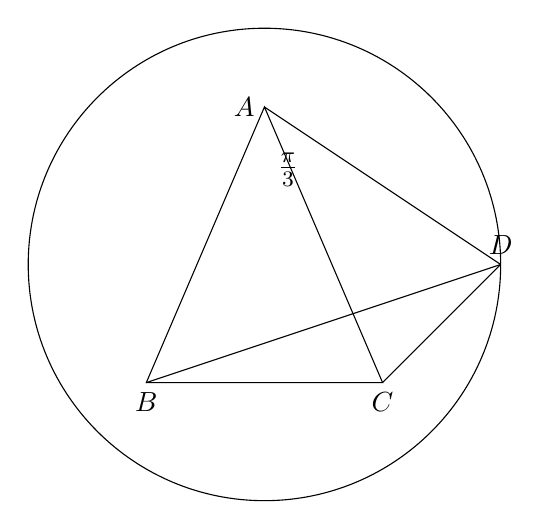
\begin{tikzpicture}
  \draw (0,0) circle (3cm);
  \coordinate [label=left:$A$] (A) at (0,2);
  \coordinate [label=below:$B$] (B) at (-1.5,-1.5);
  \coordinate [label=below:$C$] (C) at (1.5,-1.5);
  \coordinate [label=above:$D$] (D) at (3,0);

  \draw (A) -- (B) -- (C) -- cycle;
  \draw (A) -- (D);
  \draw (C) -- (D);
  \draw (B) -- (D);

  \node at (0.3,1.2) {\large $\frac{\pi}{3}$};
\end{tikzpicture}
\end{center}

\noindent
\begin{enumerate}
  \item $$\frac{54}{25}$$
  \item $\frac{117}{50}$
  \item $\frac{63}{25}$
  \item $\frac{27}{10}$
  \item $\frac{72}{25}$
\end{enumerate}

\end{document}
